\documentclass{standalone}
\usepackage{tikz}

\definecolor{quitelightgrey}{gray}{0.9}
\newcommand{\scrabbletile}[3]{
    \begin{scope}[shift={(#1)}]
        \node[draw,thick,fill=quitelightgrey,minimum size=0.9cm,rounded corners=0.1cm] at (0,0) {};
        \node at (-0.05,0) {\Large #2};
        \node at (0.35,-0.25) {\footnotesize #3};
    \end{scope}
}

\begin{document}\sffamily
    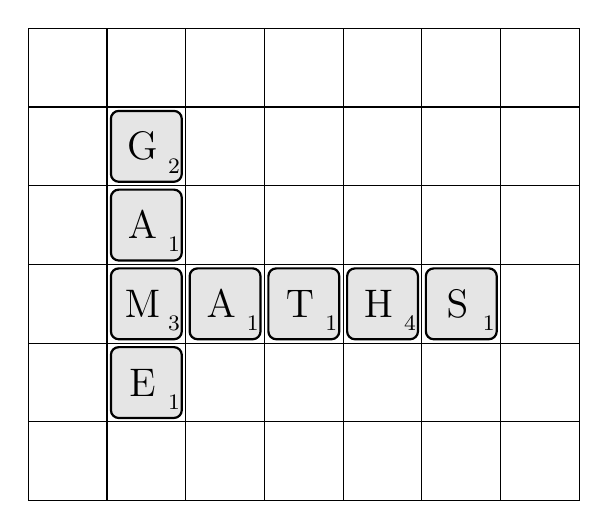
\begin{tikzpicture}
        \begin{scope}[shift={(-1.5,-0.5)}]
            \draw (0,0) grid (7,6);
        \end{scope}
        
        \scrabbletile{0,2}{M}{3}
        \scrabbletile{1,2}{A}{1}
        \scrabbletile{2,2}{T}{1}
        \scrabbletile{3,2}{H}{4}
        \scrabbletile{4,2}{S}{1}
        
        \scrabbletile{0,4}{G}{2}
        \scrabbletile{0,3}{A}{1}
        \scrabbletile{0,1}{E}{1}
    \end{tikzpicture}
\end{document}